O Acidente Vascular Cerebral (AVC) é uma das principais causas de mortalidade e incapacidade no mundo, representando um desafio crescente para os sistemas de saúde pública e para a qualidade de vida da população idosa. Segundo a Organização Mundial da Saúde (OMS), cerca de 15 milhões de pessoas sofrem um AVC a cada ano, sendo que um terço evolui para óbito e outro terço apresenta sequelas permanentes \parencite{WHO2023}. No Brasil, o AVC é a segunda principal causa de morte, com incidência especialmente elevada entre indivíduos com mais de 60 anos, faixa etária em que doenças cardiovasculares e distúrbios do ritmo cardíaco tornam-se mais frequentes \parencite{MinisterioSaude2022}.

O AVC pode ser classificado em dois tipos principais: hemorrágico e isquêmico. O tipo isquêmico, responsável por aproximadamente 85\% dos casos, ocorre quando há obstrução do fluxo sanguíneo cerebral devido à formação de coágulos, frequentemente relacionados a arritmias como a Fibrilação Atrial (FA) \parencite{JAMAAtrialFib,WJGNetStrokeRisk}. 

A Fibrilação Atrial é caracterizada por uma ativação elétrica atrial caótica, rápida e desorganizada. Em um ritmo cardíaco normal (sinusal), o Eletrocardiograma (ECG) exibe uma onda P clara antes de cada batimento, representando a contração unificada dos átrios. Na FA, essa atividade elétrica unificada desaparece; a onda P é substituída por ondas fibrilatórias irregulares (conhecidas como "ondas f"). Isso significa que os átrios deixam de contrair de forma eficaz e passam a apenas "tremular" ou "fibrilar".

Essa perda da contração atrial efetiva leva a um estado de estase sanguínea — uma lentidão significativa do fluxo de sangue — especialmente em uma pequena bolsa do átrio esquerdo chamada apêndice atrial esquerdo. Esse sangue "parado" tem alta propensão a formar trombos (coágulos sanguíneos). Quando um desses trombos se desprende, ele viaja pela artéria aorta até o cérebro, causando uma embolia cerebral e, consequentemente, o AVC isquêmico. Assim, o reconhecimento precoce de irregularidades no ritmo cardíaco é um fator decisivo para reduzir a incidência e a gravidade dos eventos cerebrovasculares \parencite{PubMedSAFARIS}.

Estudos apontam que alterações cardíacas sutis, muitas vezes assintomáticas, tendem a se manifestar durante o sono, quando o corpo entra em um estado de repouso e autorregulação fisiológica \parencite{SnifBrasil2023,JMIRContactless2024}. Nesse contexto, o monitoramento contínuo dos sinais vitais noturnos surge como uma ferramenta essencial para a vigilância clínica de idosos com risco cardiovascular elevado, especialmente aqueles que vivem sozinhos ou possuem histórico de doenças cardíacas.

Com os avanços recentes em sensores biomédicos e Internet das Coisas (IoT), tornou-se possível desenvolver dispositivos capazes de capturar e transmitir dados fisiológicos em tempo real, oferecendo suporte ao acompanhamento médico remoto \parencite{Ansys2022}. No entanto, o verdadeiro potencial dessas tecnologias está em sua integração ao trabalho médico, ampliando a capacidade de diagnóstico e prevenção por meio de informações precisas e continuamente atualizadas.

Diante dessa perspectiva, o presente projeto propõe o desenvolvimento de um sistema inteligente de monitoramento de sono voltado à prevenção de AVC em idosos, cujo foco central está tanto na captação e análise de sinais vitais durante o sono, quanto na disponibilização dessas informações ao profissional de saúde. O sistema busca fornecer ao médico um panorama detalhado do comportamento cardíaco noturno do paciente, permitindo identificar precocemente padrões de risco e embasar decisões clínicas de prevenção e tratamento. Dessa forma, pretende-se unir inovação tecnológica e relevância médica em uma solução que promova um cuidado mais humanizado, contínuo e baseado em evidências.

Além de seu caráter científico e tecnológico, o projeto também se insere no âmbito das ações de extensão universitária, em consonância com as diretrizes do Fórum de Pró-Reitores de Extensão das Instituições Públicas de Educação Superior Brasileiras (FORPROEX). Nesse contexto, contempla as áreas temáticas de Saúde e Tecnologia e Produção, e está alinhado às linhas de extensão de Desenvolvimento Tecnológico e Saúde Humana, por promover a criação de uma solução inovadora voltada à prevenção de AVC em idosos. Essa integração entre conhecimento científico, inovação e responsabilidade social reforça o compromisso da instituição com a formação cidadã e com o impacto positivo das tecnologias na melhoria da qualidade de vida da população.

\begin{center}
\captionof{figure}{Exemplo de ondas P no ECG}
\label{fig:introducao-exemplo}
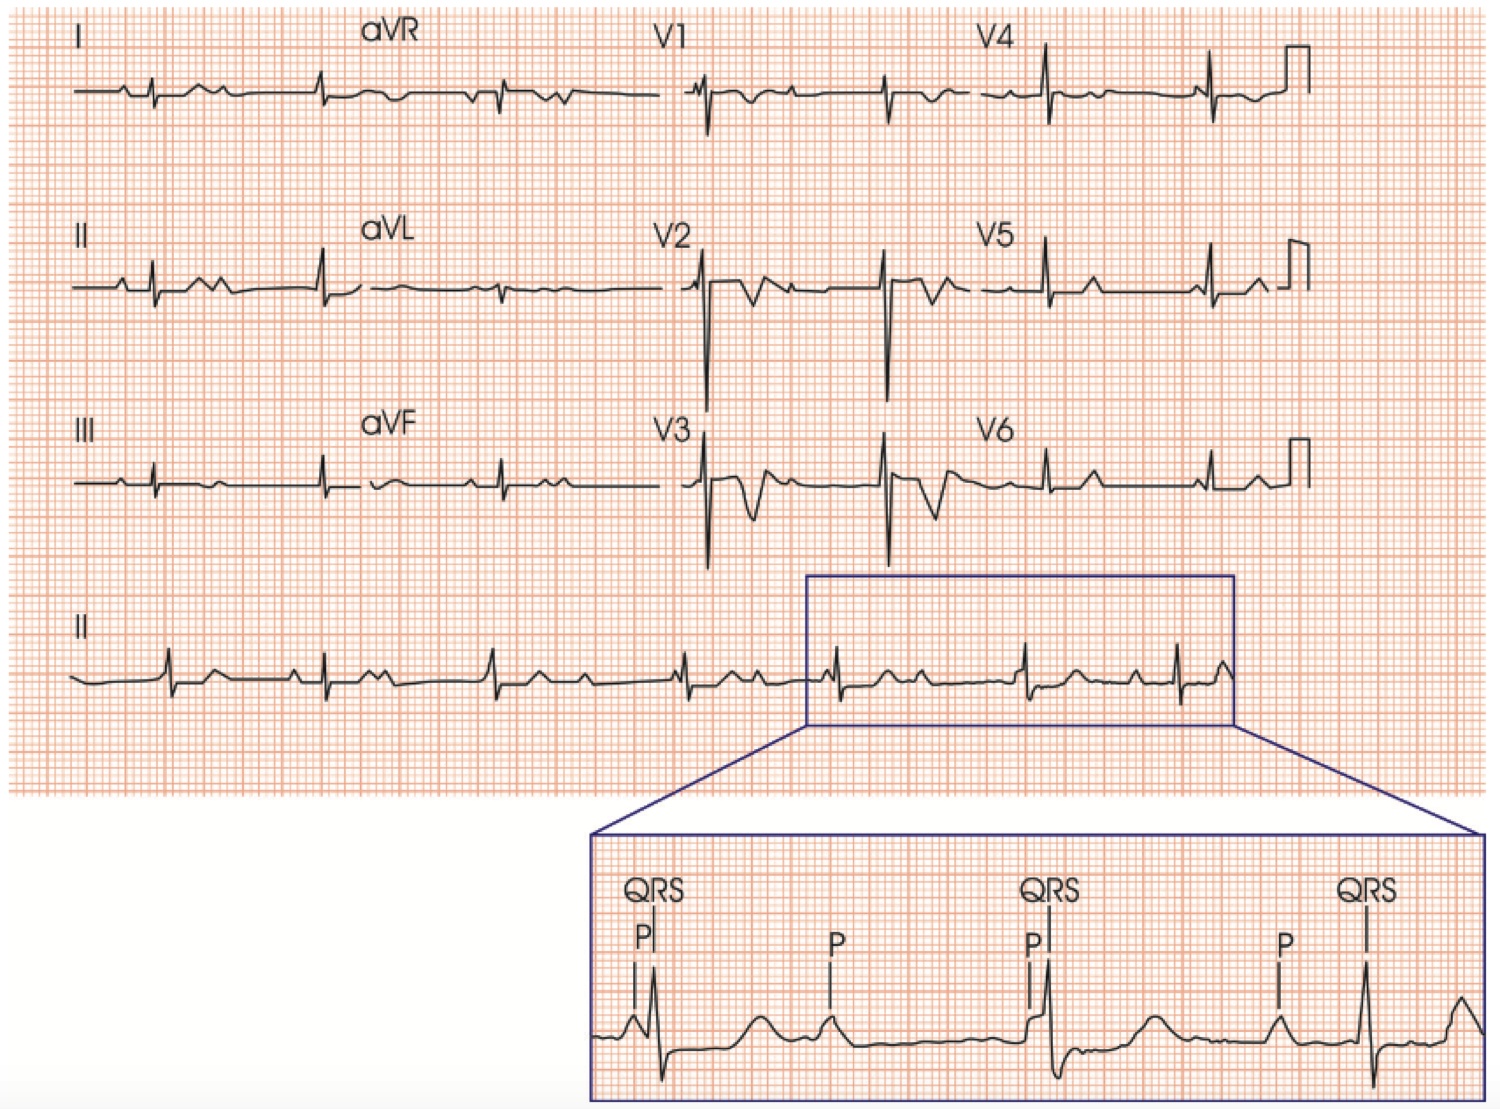
\includegraphics[width=0.8\textwidth]{Illustrations/ondas-p.png}
\vspace{1em}
\SourceOrNote{Adaptado de \textcite{PortalAfya2025}}
\end{center}

\begin{center}
\captionof{figure}{Exemplo de ondas f no ECG}
\label{fig:introducao-exemplo2}
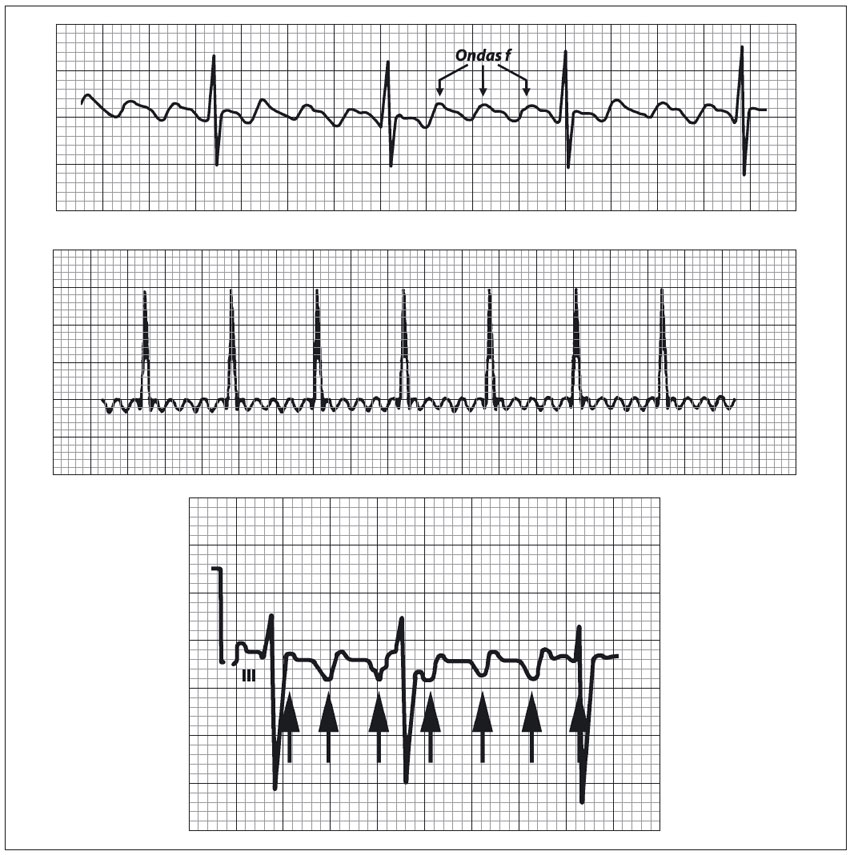
\includegraphics[width=0.7\textwidth]{Illustrations/ondas-f.jpg}
\vspace{1em}
\SourceOrNote{Adaptado de \textcite{PortalAfya2025}}
\end{center}
